
%
% foundations - spatial data
%

\section{Spatial data}

A central aspect in web mapping is dealing with spatial data. Decisions on how to structure and store spatial data highly influence the computation tasks that may be performed on such data. This mainly depends on the type of spatial data, where points are the most basic of all. Depending on the use case, different types of data are to be represented and stored: points, lines, rectangles, regions, surfaces and/or volumes. While most of the discussed concepts may be extended or generalized for processing more complex types of data, this is out of scope for this thesis. Instead, we focus on points as the most common type of spatial data~\cite{Samet90spatialdata}.

One fundamental way to store spatial data is the quadtree, a hierarchical data structure based on recursive decomposition of space. We will first discuss space orders \& decomposition and then put those in context when outlining the basics of the quadtree.

\subsection{Space order methods}

In order to store multi-dimensional, spatial data in a sequential storage like computer memory, the data needs to be serialized. Consider a pixel image as an example. Its 2-dimensional pixel values are positioned in planar space. In order to store the image, those pixels have to be processed in a predefined order, such that they can be serialized into a 1-dimensional array of memory units.

The traditional order for storing a raster of image data was row by row. The row order sequentially processes the raster row by row from left to right, starting at the top left corner. In contrast, the row-prime order switches the horizontal processing direction at the end of each row. This leads to a higher locality as it has the property of always moving to a 4-neighbor~\cite{Goodchild83raster}.

Besides the discussed row orders, additional space-ordering methods have been developed to serve different purposes. The Morton and Peano-Hilbert orders both visit entire sub quadrants first before before exiting them. The Morton order is easier to compute, because the position of each element in the ordering can be determined by interleaving the bits of the x and y coordinates of that element. The Peano-Hilbert order always moved to a 4-neighbor but is more difficult to compute. Figure~\ref{fig:space-orders} illustrates these fundamental space orders with two further ones that allow for ordering unbounded space in two (Cantor-diagonal order) or four directions (spiral order)~\cite{Samet90spatialdata}.

\begin{figure}[h]
  \begin{center}
    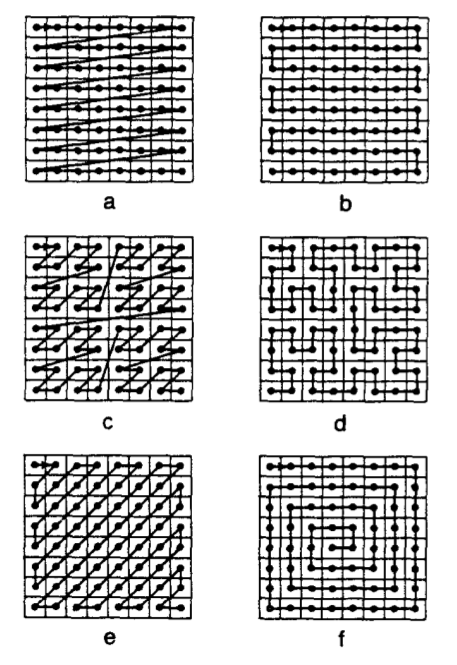
\includegraphics[width=0.5\textwidth]{figures/space_orders.png}
    \caption{The result of applying a number of different space-ordering methods to an $8 \times 8$ image whose first element is in the upper left corner of the image: (a) row order, (b) row-prime order, (c) Morton order, (d) Peano-Hilbert order, (e) Cantor-diagonal order, (f) spiral order~\cite[p 14]{Samet90spatialdata}.}
    \label{fig:space-orders}
  \end{center}
\end{figure}

The fact that the Hilbert-Peano order has the property of always moving to a 4-neighbor shouldn't be misinterpreted as still there are gaps. "A bijective mapping from multidensional data to one dimension cannot be done the way that in any case nearby multidimensional points are also close together in one dimension.~\cite{Tropf81multidimensional}". The graphic clearly shows what Samet describes as "Both the Morton and Peano-Hilbert order exhaust a quadrant or subquadrant of a square image before exiting it". This means that the orders maintain locality for those quadrants based on the hierarchy, but the edges are still disconnected. This issue will be dealt with further in Geohash (cmp. Geohash). 

\subsection{Space decomposition methods}

By definition, space decomposition methods partition space in a way so that,
\begin{itemize}
\item partitions are infinitely repetitive patterns for images of any size,
\item partitions are infinitely decomposable to generate finer sub-partitions of higher resolution.~\cite{Samet90spatialdata}
\end{itemize}

The Morton order

\subsection{Quadtree}






